%% Latex template for PhD dissertation or MS thesis
%% Department of Mechanical Engineering
%% Brigham Young University
%% Last Modified: April 2017

\documentclass[12pt,twoside]{report}% Use this line for the print version of the thesis
%\documentclass[12pt,oneside]{report}% If you comment out the line above, and uncomment this line, it will create a file without the extra pages that the Library wants for its electronic file versions.

%%%%%%%%%%%%%%%%%%%%%%%%%%%%%%%%%%%%%%%%%%%%%%%%%%%%%%%%%
%  Setup BYU thesis format
%%%%%%%%%%%%%%%%%%%%%%%%%%%%%%%%%%%%%%%%%%%%%%%%%%%%%%%%%
\usepackage{byustyle}
% Setup the byu style sheet
\byustylesetup{%
    %
    %isdissertation = true,            % Uncomment this if you're doing a PhD dissertation
    %
    % Definitions of names needed in thesis/dissertation
    deptname          = Department of Mechanical Engineering,
    committeechairman = Brian D. Jensen,
    committeemembera  = Spencer P. Magleby,
    committeememberb  = Brent W. Webb,
    graddate = April 2011,  		% Final approval month (NOT graduation month!        	
     %
    %Uncomment to shorten for proofreading purposes
    %noabstract = true,         % Don't show the abstract page
    %nouniversitypages = true,  % Don't show any of the "university pages"
    %noacknowledgements = true, % Don't show the Acknowledgements page
    %notableofcontents = true,  % Don't show the Table of Contents
    %nolistoffigures = true,    % Don't show the List of Figures
   % nolistoftables = true,     % Don't show the List of Tables
    %nonomenclature = true,     % Don't show the Nomenclature section - note that this section is optional
    %notocandlists = true,      % Don't show the Table of Contents, List of Figures, or the List of Tables
    %noheaderatall = true,      % Don't show any of the BYU Thesis header pages
    keywords = {James Watt, steam engines, nonlinear deflections, thesis templates} % Enter your keywords
%inside the curly braces, as you'd like them to appear on the bottom of the abstract page.
}
%%%%%%%%%%%%%%%%%%%%%%%%%%%%%%%%%%%%%%%%%%%%%%%%%%%%%%%%
%  Include other \usepackage{} statements here.
%    Add one package at a time.
%    Warning:  Some packages are not compatible with byuthesis.sty
%%%%%%%%%%%%%%%%%%%%%%%%%%%%%%%%%%%%%%%%%%%%%%%%%%%%%%%%%
% You should turn on any of these that you think you'll need!
%\usepackage[normalmargins]{savetrees} 	% prints smaller to save trees (draft only)
\usepackage{amsmath}										%	allows for mathematical symbols
\usepackage{amssymb}										%	defines symbol names for all the math symbols
\usepackage{graphicx}        						% for .pdf graphics inclusion
\usepackage{subfigure}									%	allows for subfigures
\usepackage{setspace}										%	change the spacing inside a document
\usepackage{epstopdf}										%	converts a .eps to a .pdf
\usepackage{cite}												%	allows for citations
\usepackage{mathptmx}
\usepackage{textcomp}
\usepackage{float}											%	improves the interface for defining floating objects
\usepackage{rotating}
%\usepackage[figuresright]{rotfloat}
%\usepackage{multirow}
%These next two lines are for the citing with the IEEE style (leave commented for ASME)
%\renewcommand\citepunct{], [}
%\renewcommand\citedash{]--[}
%%%%%%%%%%%%%%%%%%%%%%%%%%%%%%%%%%%%%%%%%%%%%%%%%%%%%%%%
% For doing bookmarks in the PDF file
%%%%%%%%%%%%%%%%%%%%%%%%%%%%%%%%%%%%%%%%%%%%%%%%%%%%%%%%%
% For more info, see:
% http://www.geocities.com/kijoo2000/latex2pdf.pdf
% http://www.tug.org/applications/hyperref/manual.html
\usepackage[pdftex,backref,pagebackref,plainpages=false]{hyperref}
\hypersetup{
    %bookmarks    = true, % Make bookmarks (default=true). This option
                          %cannot be used after package has been loaded,
                          %thus use like this: \usepackage[bookmarks=false]{hyperref}.
    %
    breaklinks   = false, % Allow link text to break across lines (default=false).
    linktocpage  = false, % make page number, not text, be link on TOC, LOF and LOT
    colorlinks   = false, % Color the text of links (true) or put color frames over
    %
    linkbordercolor  = {1 1 1}, % The color of the box around normal links (white so they won't show up)
    citebordercolor  = {1 1 1}, % The color of the box around citations (white so they won't show up)
                          % the links (false).
    pdfstartview = {FitV}, % Set the startup page view. Possible options are:
                           % FitH: Fit whole width of page
                           % FitV: Fit whole height of page
                           % FitB: Fit whole �Bounding Box� page
                           % FitBH: Fit whole width of �Bounding Box� of page
                           % FitBV: Fit whole height of �Bounding Box� of page
    bookmarksnumbered  = true, % Put section numbers in bookmarks (default=false)
    bookmarksopen      = true, % Open up the bookmark trees (default=false).
    bookmarksopenlevel = 0, % Level to which bookmarks are open (default=\maxdimen).
    bookmarkstype      = toc, % Specify which toc file to mimic (default=toc).
    pdfpagemode        = {UseOutlines}, %  Specify how document starts when opened ({None}).
                                        % Possible options are:,
                                        % None: Neither bookmarks nor thumbnails are visible.
                                        % UseOutlines: Bookmarks are visible.
                                        % UseThumbs: Thumbnails are visible.
                                        % FullScreen: Full-screen mode
    pdftitle    = {Thesis},
    pdftitle    = {Thesis Template for the Ira A. Fulton College of Engineering and Technology},
    pdfauthor   = {Iman A. Student},
    pdfcreator  = {Iman A. Student},
    pdfsubject  = {Iman A. Student's Master's Thesis},
    pdfkeywords = {Master's Thesis, BYU},
    pdfborder		=	{0 0 0},}
%%%%%%%%%%%%%%%%%%%%%%%%%%%%%%%%%%%%%%%%%%%%%%%%%%%%%%%%
%  Define macros here - You may use these, or delete them, as you see fit.
%%%%%%%%%%%%%%%%%%%%%%%%%%%%%%%%%%%%%%%%%%%%%%%%%%%%%%%%%
\def\proof{\noindent{\it Proof: }}
\def\QED{\mbox{\rule[0pt]{1.5ex}{1.5ex}}}
\def\endproof{\hspace*{\fill}~\QED\par\endtrivlist\unskip}
\newcommand{\norm}[1]{\left\|#1\right\|}
\newcommand{\abs}[1]{\left|#1\right|}
\newcommand{\defeq}{\stackrel{\triangle}{=}}
\newcommand{\re}{\mathbb{R}} 																			% real numbers
\newcommand{\OMIT}[1]{{}} 																				% omit sections of text
\newcommand{\pd}[2]{\ensuremath{\frac{\partial #1}{\partial #2}}} % partial derivative
\newcommand{\superscript}[1]{\ensuremath{^\textrm{#1}}}
\newcommand{\subscript}[1]{\ensuremath{_\textrm{#1}}}
%%%%%%%%%%%%%%%%%%%%%%%%%%%%%%%%%%%%%%%%%%%%%%%%%%%%%%%%
% To only print a few chapters without changing the reference numbers, 
%		uncomment the chapters you want
%%%%%%%%%%%%%%%%%%%%%%%%%%%%%%%%%%%%%%%%%%%%%%%%%%%%%%%%
%\includeonly{chapter1}
%\includeonly{chapter2}
%\includeonly{chapter3}
%\includeonly{chapter4}
%\includeonly{chapter5}
%\includeonly{chapter6}
%\includeonly{chapter7}
%\includeonly{appendixa}
%\includeonly{appendixb}
%\includeonly{appendixc}
%\includeonly{appendixd}

%%%%%%%%%%%%%%%%%%%%%%%%%%%%%%%%%%%%%%%%%%%%%%%%%%%%%%%%
% Start Document
%%%%%%%%%%%%%%%%%%%%%%%%%%%%%%%%%%%%%%%%%%%%%%%%%%%%%%%%
\begin{document}

% Define Title & Author
% For a title of more than one line, use the \\ to break up the lines so they appear in an inverse pyramid shape.
%Also, make sure you use title case (upper case for most of the first letters of words)
\title{Thesis Template for the Mechanical Engineering Department}%Ira A. Fulton College\\ of Engineering and Technology}
\author{Iman A. Student}

% For displaying the BYU Thesis header
% 	This command assumes that there are documents called abstract.tex and
% 	acknowledgements.tex that will be included in the header
\showBYUHeader

% Include chapters of the thesis here: (Note that you should open the files chapter1.tex and chapter2.tex to
% see some of the important notes about how to do your thesis!)
\chapter{Introduction}
\label{chp:chapter1}
\graphicspath{{figures/}{figures/chapter1/}}
This is an example of the introduction. It's pretty simple and shows off
some of the basic commands.

\section{First Section}
This part shows how you can divide things into sections.

\subsection{First Subsection}
Also into subsections.

\subsection{Second Subsection}
Which really helps organization and automatically gets added to the Table
of Contents and gets linked to by the hyperref package.

\section{Citation Example}
One of the greatest parts about \LaTeX\ is BibTeX. You can just call
the $\backslash$cite command and it will organize the whole references section for you as long as there is an entry in the refs.bib file (or whichever other .bib file you tell it to use; see the source for master.tex).
Here is an example of citing previous works
\cite{guy06best,guy06second}.

\section{Fixed Width Figure Example} \label{sec:intro_figure_example}
This part also shows how to include a basic figure like the ones
shown in Figures~\ref{fig:intro_stuff2} and \ref{fig:intro_stuff}. %Figure~\ref{fig:example} illustrates the use of a figure placed in landscape.
\begin{figure}[t]
  \centering
  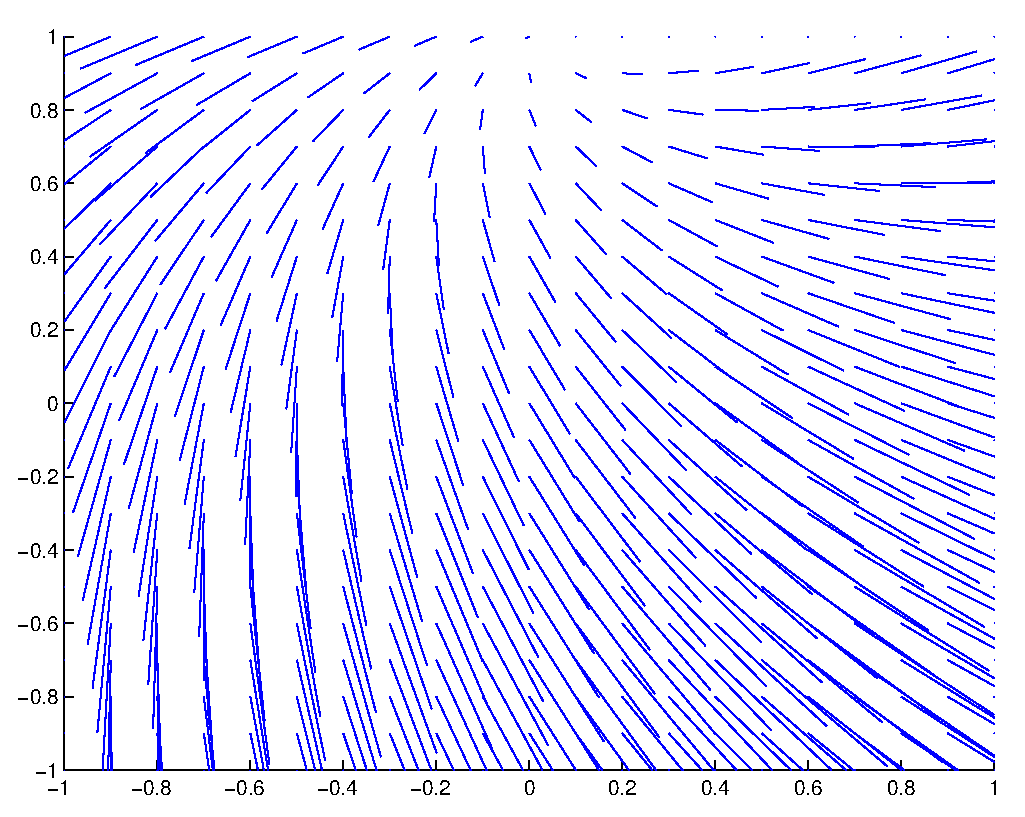
\includegraphics[width = 2in]{stuff}
  \caption[Example small width figure]{
Example small width figure, showing how to use the width option.}
%
  \label{fig:intro_stuff2}
\end{figure}

\begin{figure}[t]
  \centering
  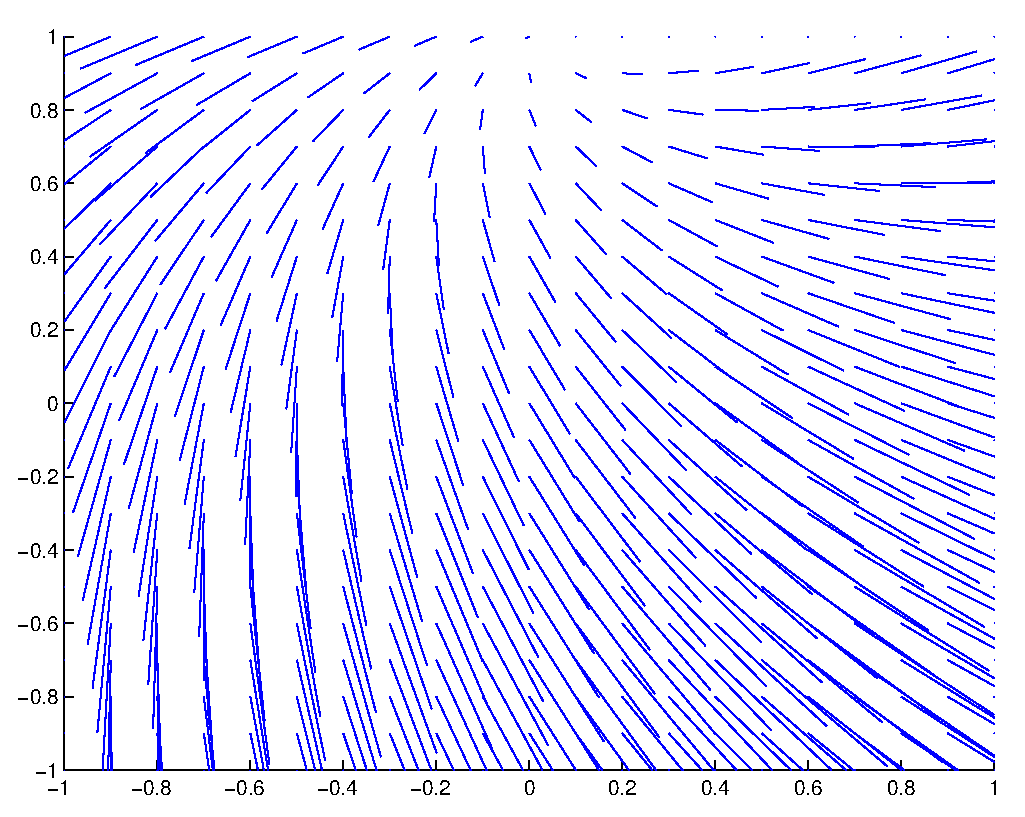
\includegraphics[width=5.5in]{stuff}
  \caption[Example fixed width figure]{
This figure is just a simple figure with a width set at 5.5~in. An example of a
figure whose size depends on the width of the page is given in
Figure \ref{fig:appendix_some_pic} in Section~\ref{sec:appendixa_figure_example} of Appendix~\ref{apdx:appendixa}.}
%
  \label{fig:intro_stuff}
\end{figure}

%\begin{sidewaysfigure}[p]
%\includegraphics[scale=0.8]{examplegraphic}
%\caption{An example of a landscape graphic.}
%\label{fig:example}
%\end{sidewaysfigure}

\section{Math and Equation Example, Where the Heading Is Made so Long That It Extends onto a Second Line}
Here is how to use inline math mode to define lambda like this,
$\lambda$, and how to declare Equations~\eqref{eqn:definition_Ix}
and~\eqref{eqn:definition_Iy}

\begin{equation} \label{eqn:definition_Ix}
I_x(x,y) = \pd{I(x,y)}{x},
\end{equation}

\begin{equation}\label{eqn:definition_Iy}
I_y(x,y) = \pd{I(x,y)}{y}.
\end{equation}

 Or you can create equation arrays like
\begin{align}
  \alpha &= \beta^\gamma \\
  x &= \frac{1}{\alpha} \label{eq:cool_1} \\
  y &= \sqrt{\abs{\frac{\gamma}{\beta}}}  \\
  \zeta &= x^y \label{eq:cool_2}.
\end{align}


The lines in the array can be referenced by saying things like: In
Eqn.~\eqref{eq:cool_1} we show a wonderful equation, but it's not nearly as
amazing as Eqn.~\eqref{eq:cool_2}.

\chapter{Making Tables}
\label{chp:chapter2}
\graphicspath{{figures/}{figures/chapter2/}}

\section{Making a Table}
An example \LaTeX\ table is shown below in Table~\ref{tab:comparison}.
You make a table by starting a table environment with a caption
and label.  You can specify the text that shows up in the Table of
Contents using the optional parameter box, [], that's at the
beginning of the $\backslash$caption command. You tell the table how
many columns in the beginning of the tabular environment using a
command like this: $|$ l $|$ c $|$ r $|$. That would create a table with 3 columns
that are left-aligned, centered and right-aligned, in that order. The $|$'s tell \LaTeX\ that
you want bars separating the columns. Of course, you can also make tables without the $|$ characters, in which case no lines will be added between the fields, which often looks better. You can also add horizontal
lines using the $\backslash$hline command. This example is also centered in the page using the
$\backslash$centering command.
%
\begin{table}[b]
\centering
\caption[Example table]{Description of the table, where the caption is long enough\\ to go onto more than one line. You should put line breaks in to\\ make the caption not extend beyond the edges of the table,\\ and to make an ``inverted pyramid.''}
\label{tab:comparison}
%
\begin{tabular}{|l|c|c|r|}
\hline

Table Name  & Column 2 & Column 3   & Column 4 \\
\hline
First Row   & 4780286  & 72.941376  & A \\
Second Row  & 4069335  & 62.093124  & B \\
Third Row   & 4074900  & 62.178040  & C \\
\hline
Fourth Row  & 4000000  & 60.000000  & Z \\
\hline

\end{tabular}
\end{table}
%

Landscape tables can also be inserted, if desired, using the \verb-sidewaystable- environment, which is defined in the \verb!rotating! package. An example is found on the next page, in Table~\ref{tab:landscape}. Note that landscape tables and figures should be the exception rather than the rule, since they are more awkward to read. However, if you have an especially wide table or figure that cannot be reduced in size without losing required resolution, placing it in landscape may be a good idea.
\begin{sidewaystable}
\caption{A landscape table}\vspace*{6pt}
\label{tab:landscape}
\setlength{\tabcolsep}{6mm}
\begin{tabular}{lcccc}
Year & Method of CVD Deposition & Thickness ($\mu$m) & Hardness (MPa) & Resistivity ($\Omega\cdot$m)\\ 
\hline\\[-11pt]
1999 & LPCVD & 5.1 & 175 & 2.3$\times10^{-5}$\\
2000 & PECVD & 17.2 & 101& 1.5$\times10^{-5}$\\
2002 & PECVD & 4.3 & 55 & 3.4$\times10^{-5}$\\
2004 & LPCVD & 1.1 & 225 & 5.1$\times10^{-5}$\\
\hline
\end{tabular} 
\end{sidewaystable}

%%%%%%%%%%%%% begin Bibliography %%%%%%%%%%%%%%%%%
\cleardoublepage
\bibliographystyle{asmems4}%Change this to use a different bibliography style, such as ieeetran.
\bibliography{refs}% Change this to use a different bibliography database file.

% Include appendix sections here: (or comment these lines out to have no appendices)
\appendix
\chapter{Making a Figure with Width Based on Page Size}
\label{apdx:appendixa}
\graphicspath{{figures/}{figures/appendixa/}}

\section{Width Based on Page Size Figure Example} \label{sec:appendixa_figure_example}
Here's an example of a figure whose width depends on the width
of the page. You can see it as Figure~\ref{fig:appendix_some_pic}. This also shows another citation \cite{aeyels86local}.

\begin{figure}[htbp]
  \centering
  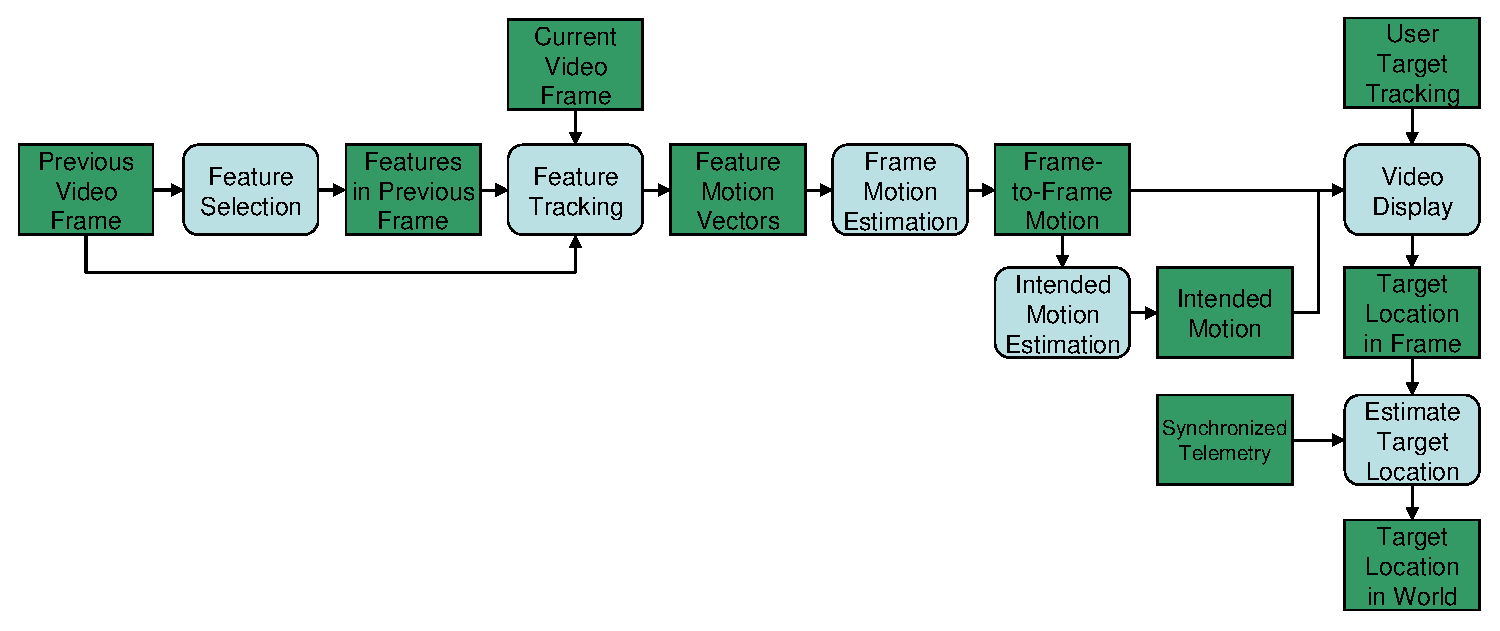
\includegraphics[width=0.45\textwidth]{some_pic}
  \caption[Example figure whose width depends on page size]{
    This is an example of a figure whose width will be 45\% of the
    width of the page. If you'd like to see a figure with a fixed
    width then you can see it as Figure~\ref{fig:intro_stuff} in
    Section~\ref{sec:intro_figure_example} of Chapter~\ref{chp:chapter1}.}
  \label{fig:appendix_some_pic}
\end{figure}
\chapter{Formatting Guidelines for Thesis}
\label{apdx:appendixb}

This appendix outlines the required formatting for theses and dissertations. While the \LaTeX\ template takes care of most of these automatically, it is the student's responsibility to ensure that all formatting requirements are incorporated in the document.

\section{Font} Times New Roman 12 pt. throughout text and 10 or 11 point for tables and figures.

\section{Margins}
\begin{itemize}
\item Preliminary Pages (Title page, Abstract page(s), Acknowledgment page, Table of Contents, List of Figures, List of Tables):
1 inch on all sides
\item Body Pages, beginning with Introduction:
1 inch on all sides
\item Chapter title pages, Appendix title page, Reference title page:
2 inches at top,
1 inch at bottom and sides
\end{itemize}

\section{Printing}
\begin{itemize}
\item Single-sided: Title page, Abstract page(s), Acknowledgment page
\item Two-sided:  Table of Contents, List of Figures, List of Tables, Body, Appendix, References
\end{itemize}
Note:  Table of Contents, List of Figures, List of Tables, Chapter title pages, References and Appendix pages must begin on the front side of a page.

\section{Page Numbering}
\begin{itemize}
\item	Page numbers are centered at the bottom of the page.
\item	Counting begins with the Title page; however, back pages are not counted until the Table of Contents.
\item	Page numbers do not appear on the page until the Table of Contents (v).
\item	Use Roman Numerals (v, vi, vii, ...) for the Table of Contents page and the pages thereafter until Chapter 1.  
\item	Use Arabic numbers (1, 2, 3 ...) beginning with Chapter 1. 
\item	Be sure numbers appear on all blank back pages once numbering begins.
\end{itemize}

\section{Spacing}
\begin{itemize}
\item	Double-space text of body.
\item	Single-space abstract, captions, quotes, long chapter titles, headings, and subheadings.
\item	Table of Contents, List of Figures, List of Tables, and References can be single-spaced or double spaced.
\item	Double-space three times after chapter titles (48 pts).
\item	Double-space twice before subheadings (24 pts). 
\item	Double-space once after subheadings (0 pts). 
\item	Double-space once between two subheadings (0 pts). 
\item	Double-space twice before and after figures (24 pts).
\item	Double-space twice before and after tables (24 pts).
\item	Double-space once before and after equations (0 pts).
\item	Do not leave a single line of text, a single-line equation, or a subheading alone on the top (widow) or bottom (orphan) of a page.
\item	Do not leave more than about 5 lines of white space remaining on a page unless it�s the end of a chapter.
\end{itemize}

\section{Figures}
\begin{itemize}
\item	Figures are normally diagrams, graphs, maps, or charts.
\item	Center figures on the page.
\item	Center captions below the figure. If two lines are needed, the caption should be left justified at margin.
\item	A figure should be placed after the paragraph of reference.  If it will not fit on the same page, continue the text and place the figure on the next page.
\end{itemize}

\section{Tables}
\begin{itemize}
\item	Tables contain numerical or statistical information.
\item	Center tables on the page.
\item	Center captions above the table.  If more than one line is needed, center the lines in an inverted pyramid:                                                          
\begin{center}Table 6.3 Comparison of roll rotation plots when node was displaced,\\
 and an X-direction off-axis force was applied.\end{center}
\item	If placed in the landscape position, the top of the table should be on the left side of the page, with the caption above the table.  The page number is placed in the standard location.
\end{itemize}

\end{document}